\subsection{Progettazione Architetturale}
\label{progettazione_architetturale}
\textbf{Durata:} dal 2020-01-19 al 2020-03-01
\\La Progettazione Architetturale inizia appena concluso il periodo precedente e termina con la Revisione di Progettazione.

Le \glo{precondizioni} sono:
\begin{itemize}
    \item Le \glo{postcondizioni} del periodo precedente sono state soddisfatte;
    \item La candidatura del gruppo al progetto {\NomeProgetto} è stata accolta.
\end{itemize}

Le postcondizioni sono:
\begin{itemize}
    \item Aggiornamento e correzione dei documenti già prodotti;
    \item Produzione del \textit{Proof of Concept} e dell'Allegato Tecnico;
    \item Completamento della progettazione ad alto livello del software;
    \item Consegna dei documenti richiesti in entrata alla \textit{Revisione di Progettazione};
    \item Ultimata preparazione della presentazione da esporre in sede di revisione.
\end{itemize}
Le attività da svolgere durante il periodo sono:
\begin{itemize}
    \item \textbf{Incremento e Verifica:} i documenti già prodotti vengono migliorati e aggiornati se necessario (\textit{\NdP}, \textit{\PdP}, \textit{Glossario},\textit{\PdQ}, \textit{\AdR});
    \item \textbf{Technology Baseline:} viene fatta un'analisi ad alto livello del software e viene redatto l'Allegato Tecnico dove vengono individuati i design pattern che verranno adottati per lo sviluppo. Infine viene codificato il \glo{\textit{Proof of Concept}}, il quale viene presentato o condiviso al committente e proponente in una data da definirsi. Il gruppo ipotizza di riuscire a sviluppare il {\textit{Proof of Concept}} attraverso due incrementi:
    \begin{itemize}
        \item \textbf{Incremento 1 (dal 2020-02-12 al 2020-02-18)}: In questo periodo l'obiettivo principale è riuscire a implementare i requisiti e i casi d'uso fondamentali concordati con l'utente sotto forma di codice;
        \item \textbf{Incremento 2 (dal 2020-02-19 al 2020-02-26)}: Realizzazione dei requisiti e dei casi d'uso non completati precedentemente e miglioramento di quelli già implementati.
    \end{itemize}
\end{itemize}

\newpage
\subsubsection{Diagramma di Gantt: Progettazione Architetturale}

\begin{figure}[ht]
    \centering
    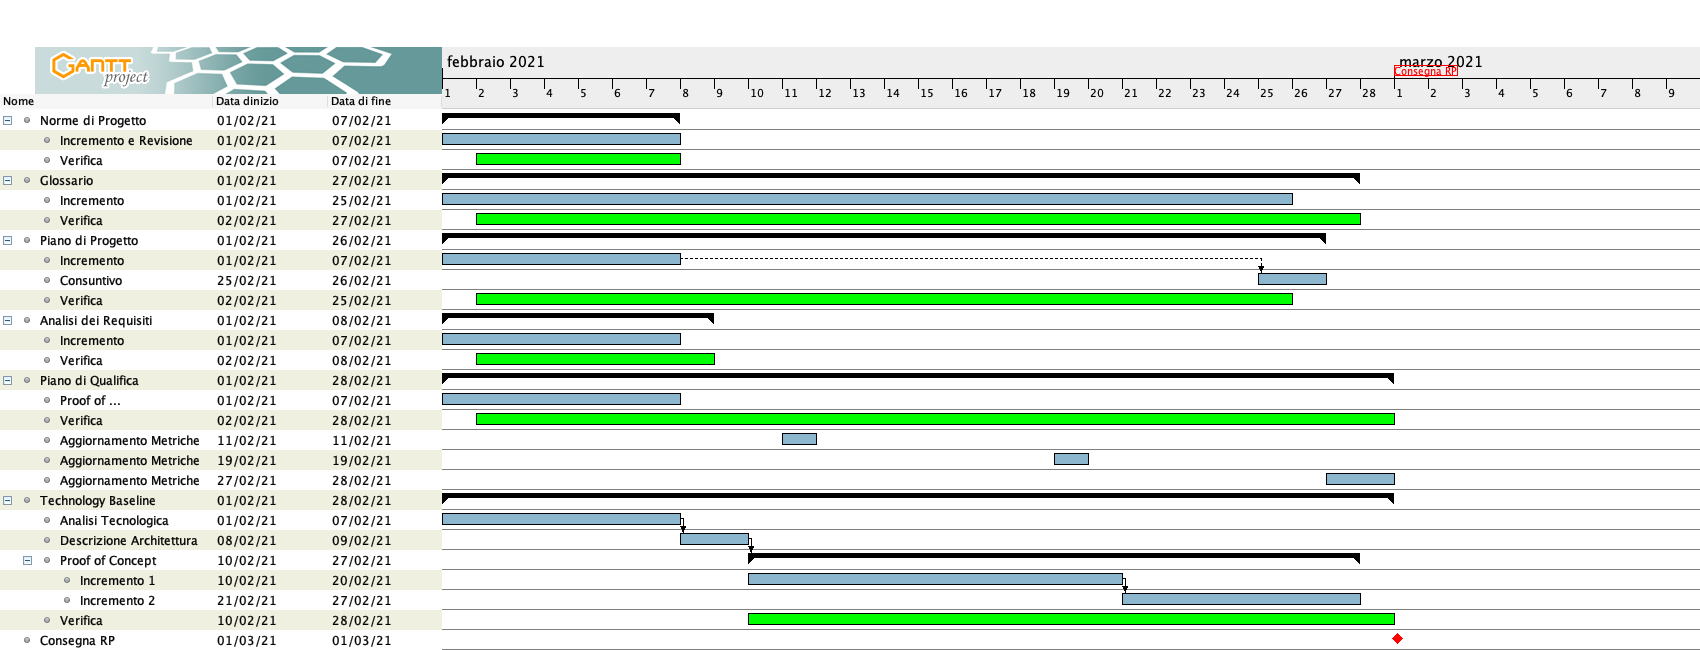
\includegraphics[width=\textwidth]{../../Immagini/GanttProgettazioneArchitetturale}
    \caption{Diagramma di Gantt dell'avvitià di Progettazione Architetturale}
\end{figure}